\section{Code Reviews}
Wie in der Beschreibung des Qualitätsziels "`Korrektheit"' bereits beschrieben, wurden nach der Implementierung einer Userstory
der Code gesichtet und mithilfe einer Checkliste bewertet. Diese enthielt die folgenden Anforderungen:
\begin{itemize}
	\item Test Coverage (auf unseren Dateien) mindestens 90\%
	\item Jede Klasse und Funktion ist grob Dokumentiert
	\item Schwierige Codestellen sind dokumentiert
	\item Alle Test laufen fehlerfrei durch
	\item Der Code ist korrekt formatiert
	\item Code erfüllt das Akzeptanzkriterium der Userstory (und dabei spezifisch nur das Akzeptanzkriterium dieser Userstory)
	\item Die Userstory ist ausgefüllt (Datum, Zeit)
\end{itemize}
Alle Checklisten sind vollständig ausgefüllt, da nicht erfüllte Punkte dem zuständigen Entwickler direkt mitgeteilt wurden und, nach Behebung, entsprechend
angehakt wurden.
Es folgen die ausgefüllten Checklisten. Da die ersten beiden Userstorys in gemeinsamer Arbeit entstanden sind, gibt es keine Checkliste dafür.

\begin{tabular}{|l|l|l|}
        \hline
        User Story & Reviewer & Datum \\
        \hline
         & & \\
        \hline
\end{tabular}

\begin{figure}[H]
\centering
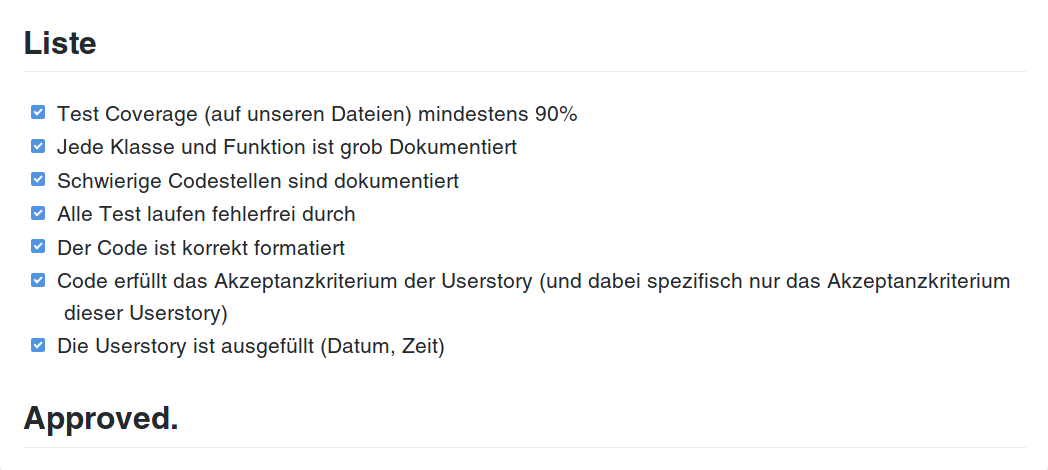
\includegraphics[width=.8\textwidth]{code_review/us03}
	\caption{Review zur Userstory 3}
\end{figure}

\begin{figure}[H]
\centering
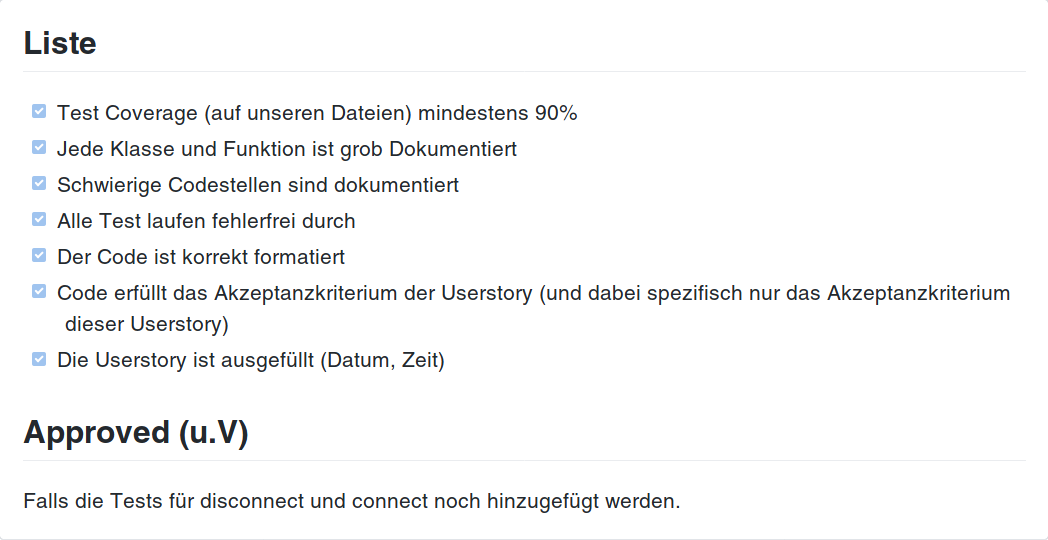
\includegraphics[width=.8\textwidth]{code_review/us04}
\caption{Review zur Userstory 04}
\end{figure}

\begin{figure}[H]
\centering
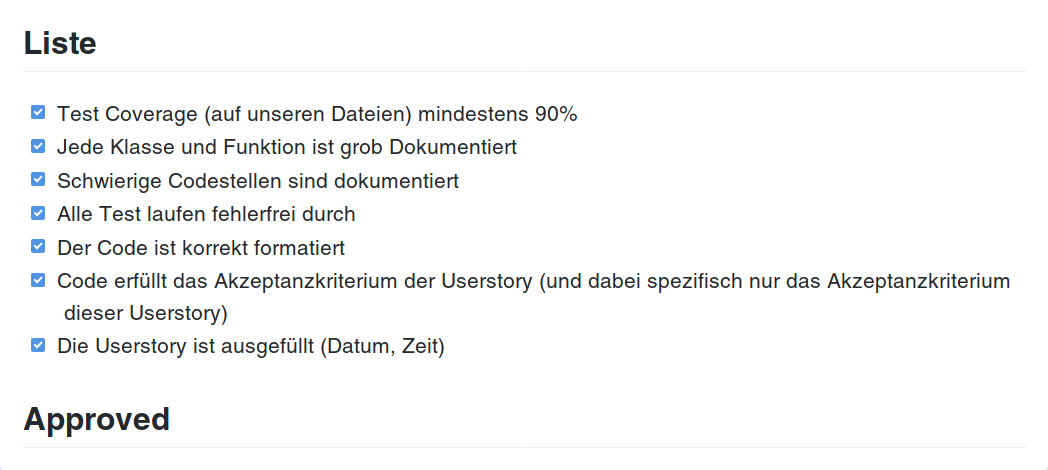
\includegraphics[width=.8\textwidth]{code_review/us05}
\caption{Review zur Userstory 05}
\end{figure}

\begin{figure}[H]
\centering
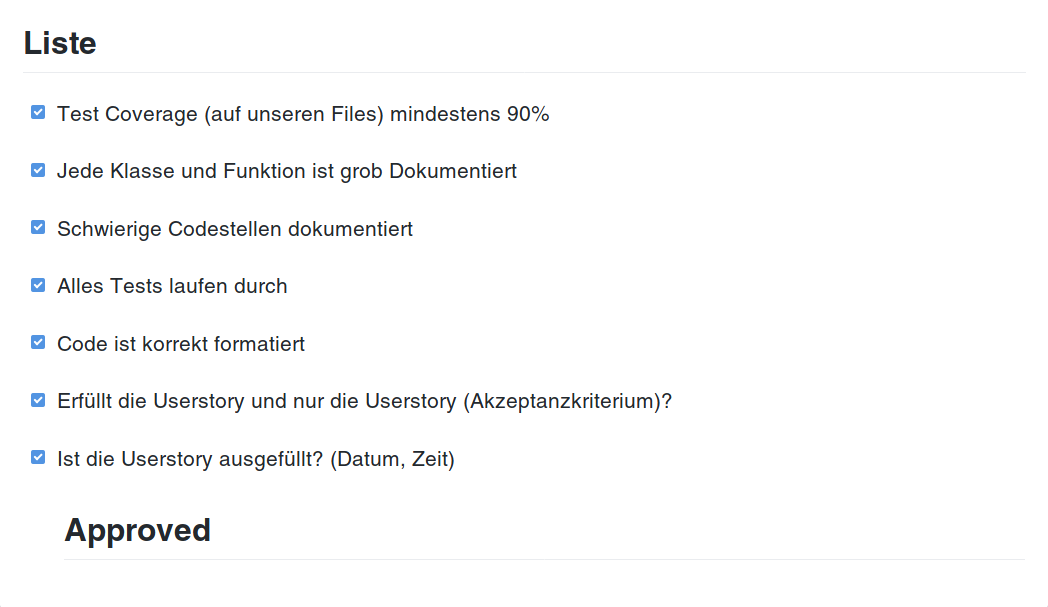
\includegraphics[width=.8\textwidth]{code_review/us06}
\caption{Review zur Userstory 06}
\end{figure}

\begin{figure}[H]
\centering
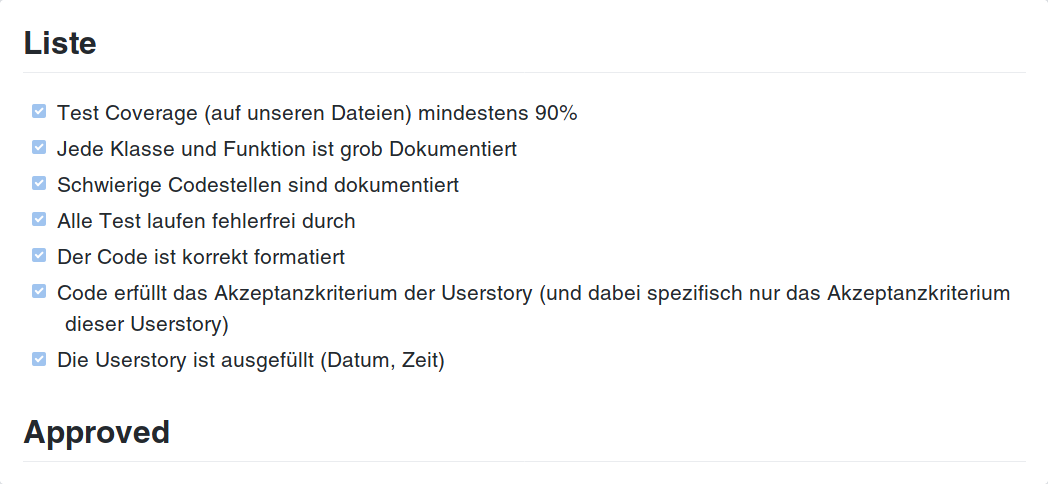
\includegraphics[width=.8\textwidth]{code_review/us07}
\caption{Review zur Userstory 07}
\end{figure}

\begin{figure}[H]
\centering
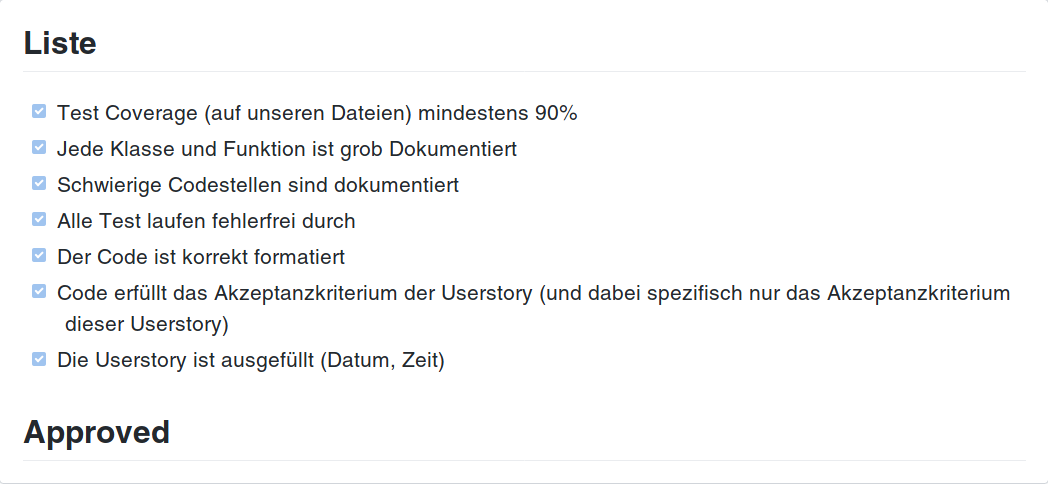
\includegraphics[width=.8\textwidth]{code_review/us08}
\caption{Review zur Userstory 08}
\end{figure}

\begin{figure}[H]
\centering

\includegraphics[width=.8\textwidth]{code_review/us09}
\caption{Review zur Userstory 09}
\end{figure}

\begin{figure}[H]
\centering
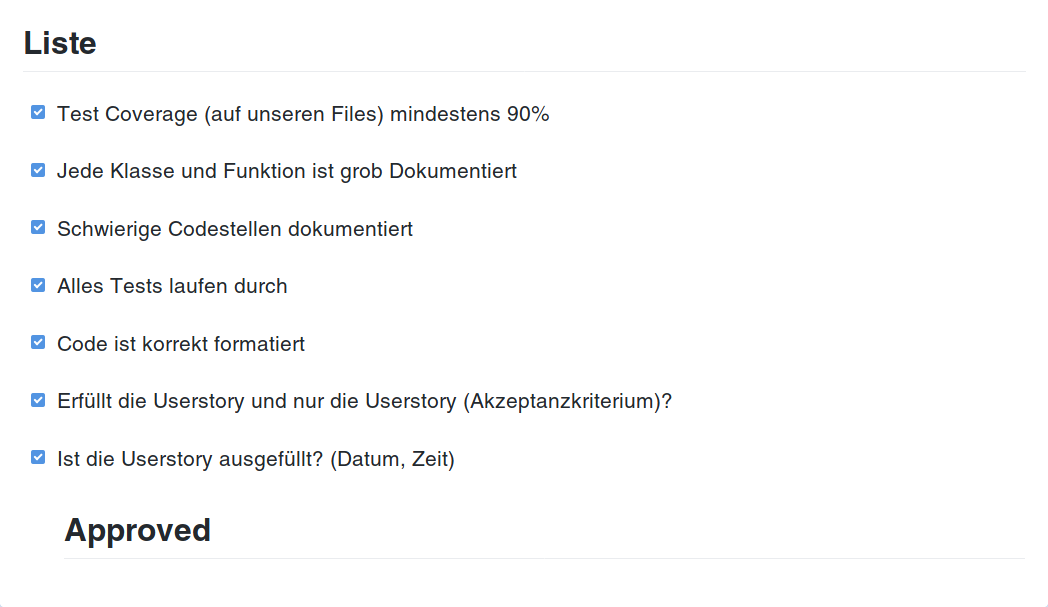
\includegraphics[width=.8\textwidth]{code_review/us14}
\caption{Review zur Userstory 14}
\end{figure}

\begin{figure}[H]
\centering
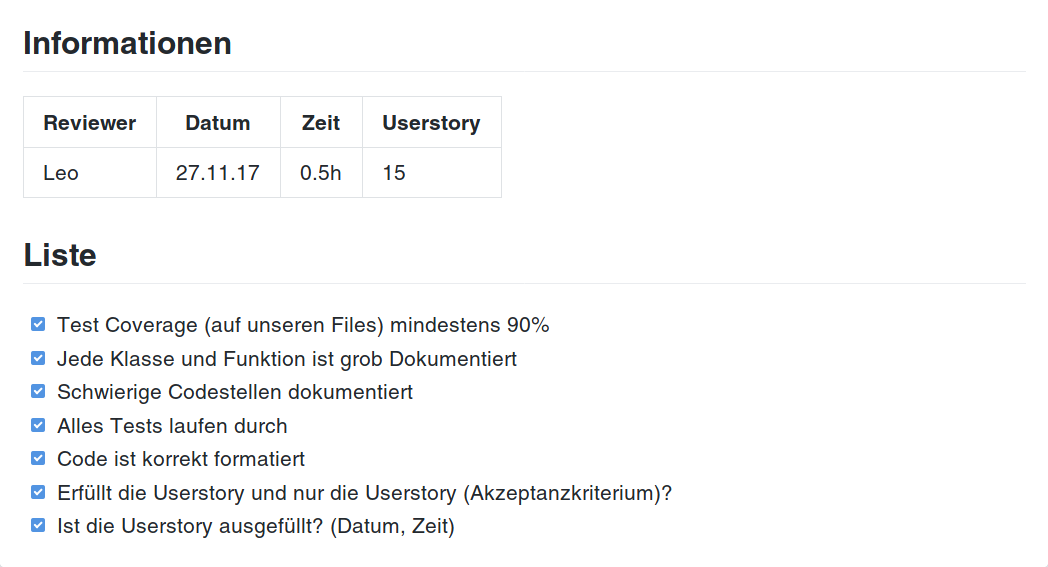
\includegraphics[width=.8\textwidth]{code_review/us15}
\caption{Review zur Userstory 15}
\end{figure}

\begin{figure}[H]
\centering
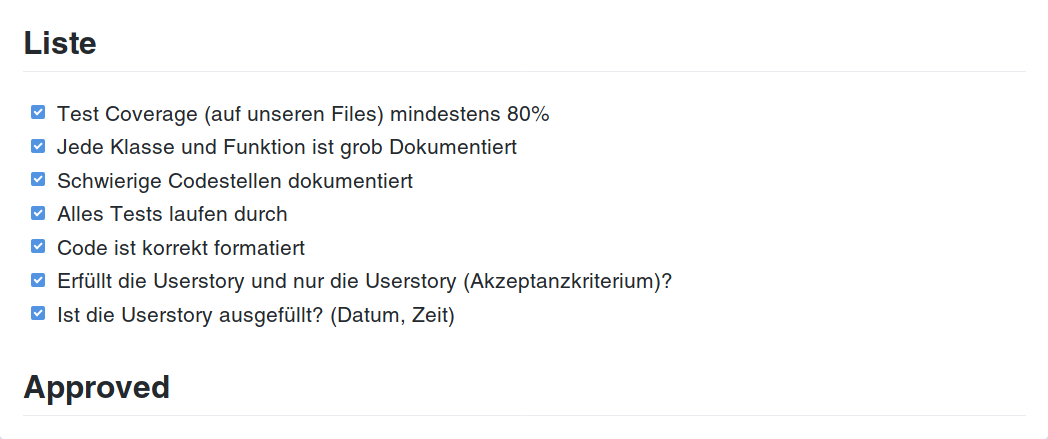
\includegraphics[width=.8\textwidth]{code_review/us16}
\caption{Review zur Userstory 16}
\end{figure}

\begin{figure}[H]
\centering
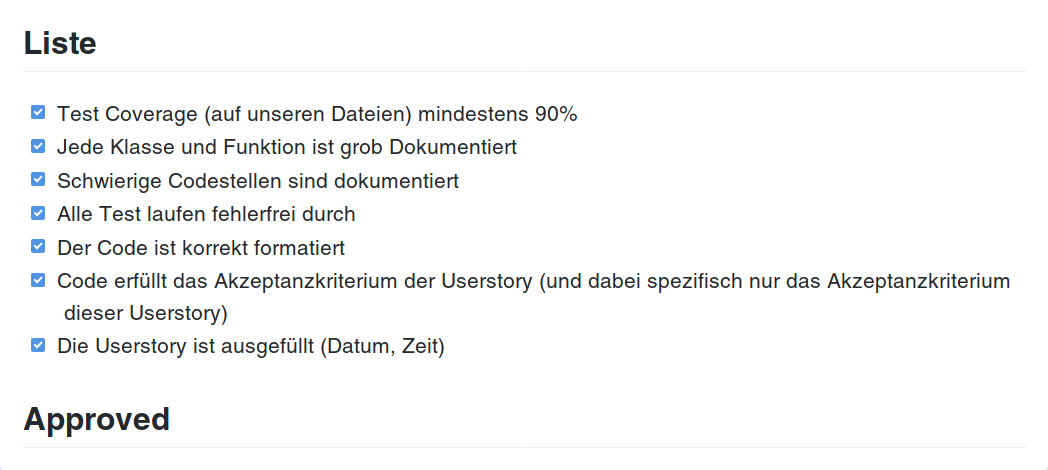
\includegraphics[width=.8\textwidth]{code_review/us17}
\caption{Review zur Userstory 17}
\end{figure}

\begin{figure}[H]
\centering
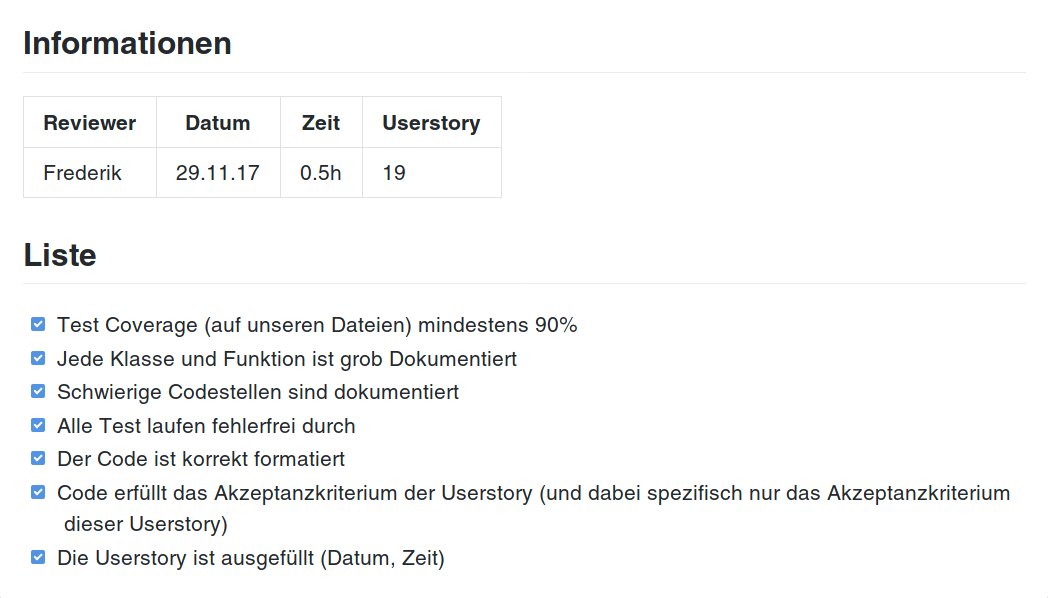
\includegraphics[width=.8\textwidth]{code_review/us19}
\caption{Review zur Userstory 19}
\end{figure}

\begin{figure}[H]
\centering
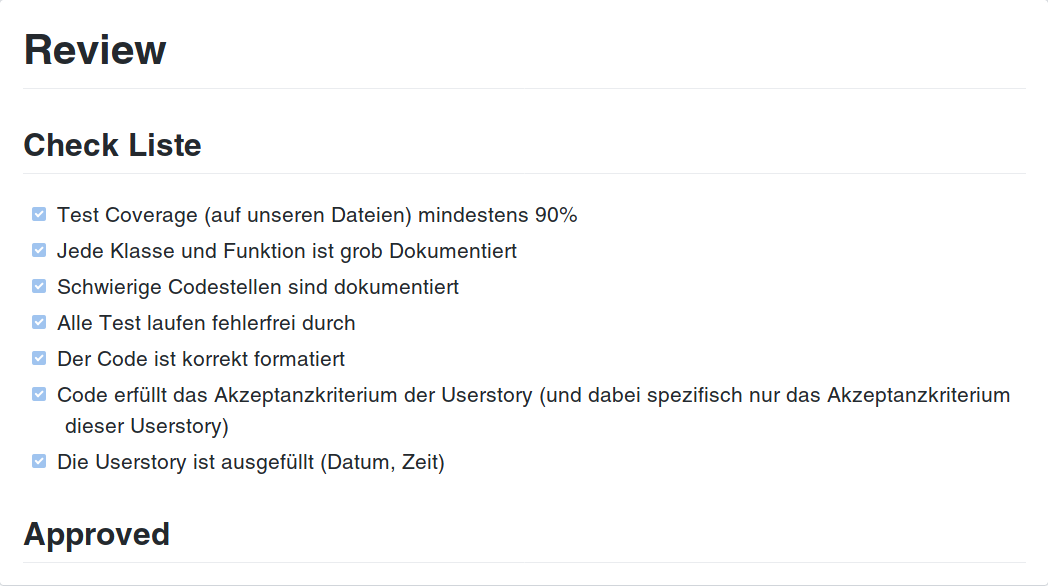
\includegraphics[width=.8\textwidth]{code_review/us20}
\caption{Review zur Userstory 20}
\end{figure}

\begin{figure}[H]
\centering
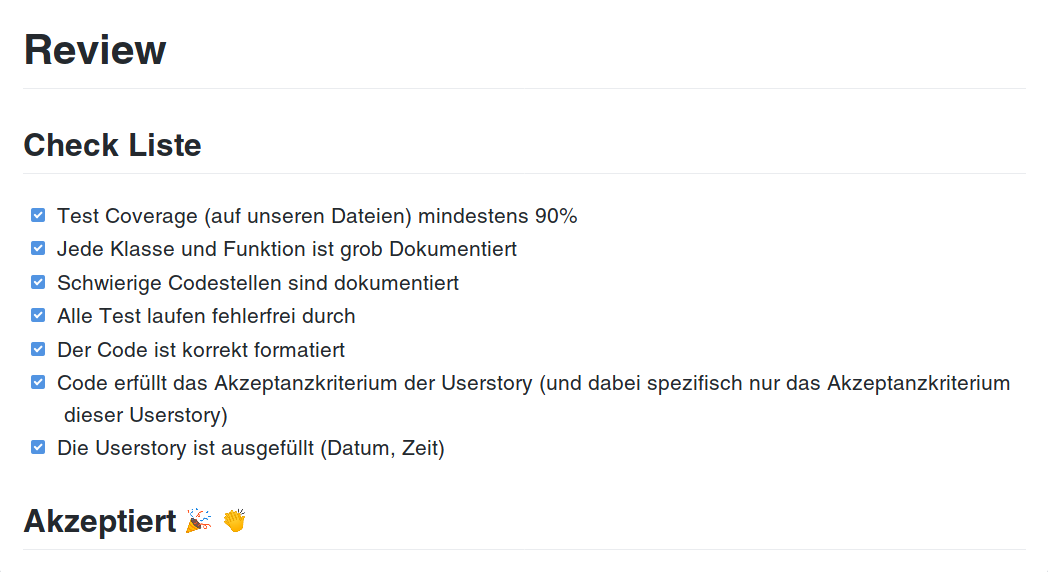
\includegraphics[width=.8\textwidth]{code_review/us21}
\caption{Review zur Userstory 21}
\end{figure}

\begin{figure}[H]
\centering
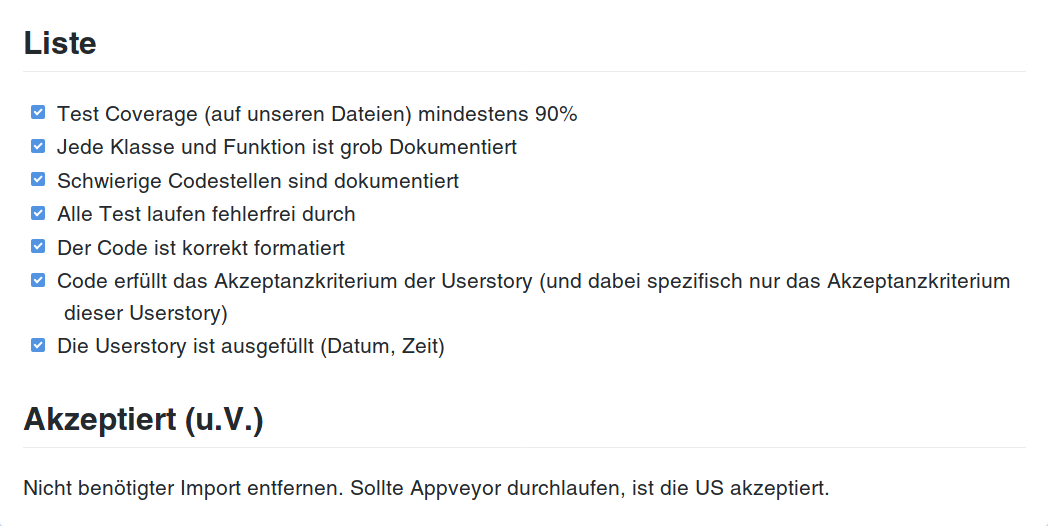
\includegraphics[width=.8\textwidth]{code_review/us22}
\caption{Review zur Userstory 22}
\end{figure}

\begin{figure}[H]
\centering

\includegraphics[width=.8\textwidth]{code_review/us23}
\caption{Review zur Userstory 23}
\end{figure}

\begin{figure}[H]
\centering
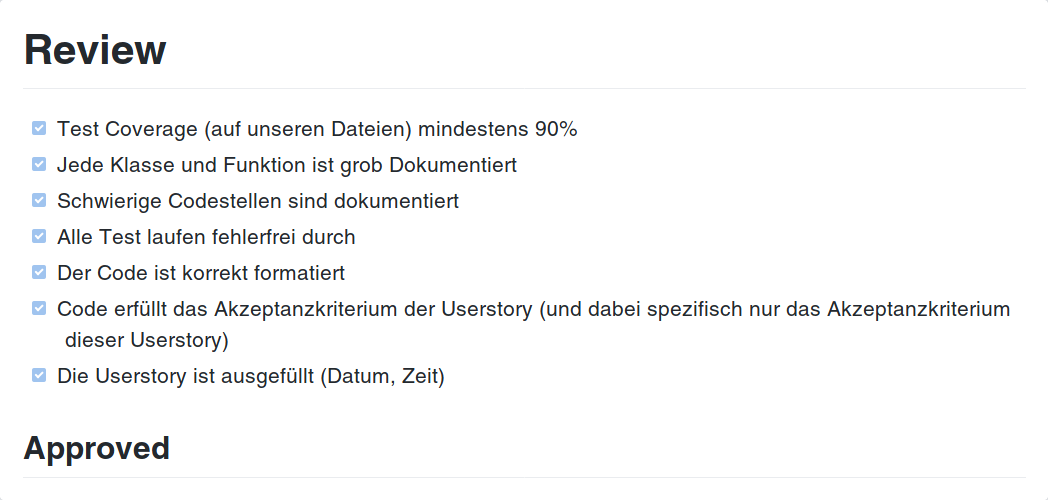
\includegraphics[width=.8\textwidth]{code_review/us24}
\caption{Review zur Userstory 24}
\end{figure}

\begin{figure}[H]
\centering
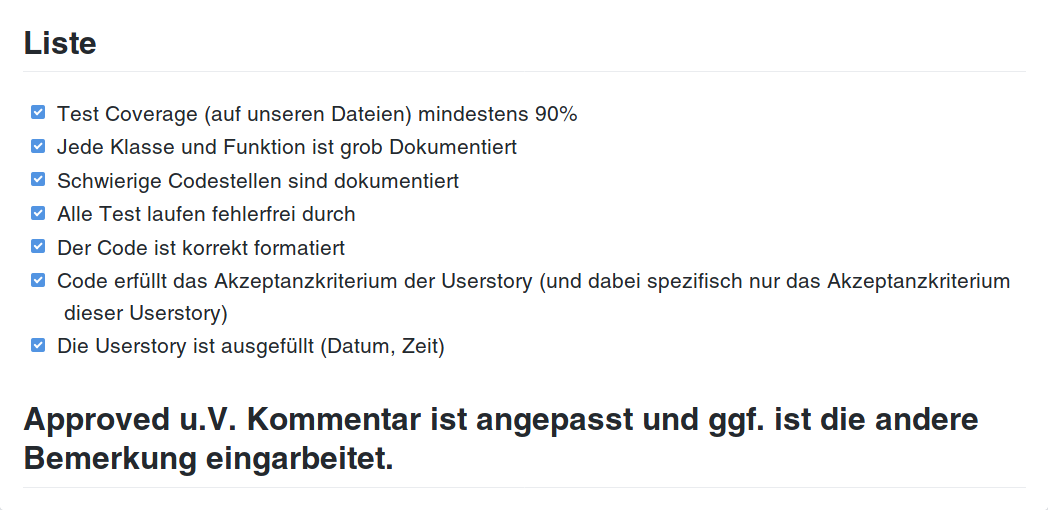
\includegraphics[width=.8\textwidth]{code_review/us25}
\caption{Review zur Userstory 25}
\end{figure}

\begin{figure}[H]
\centering
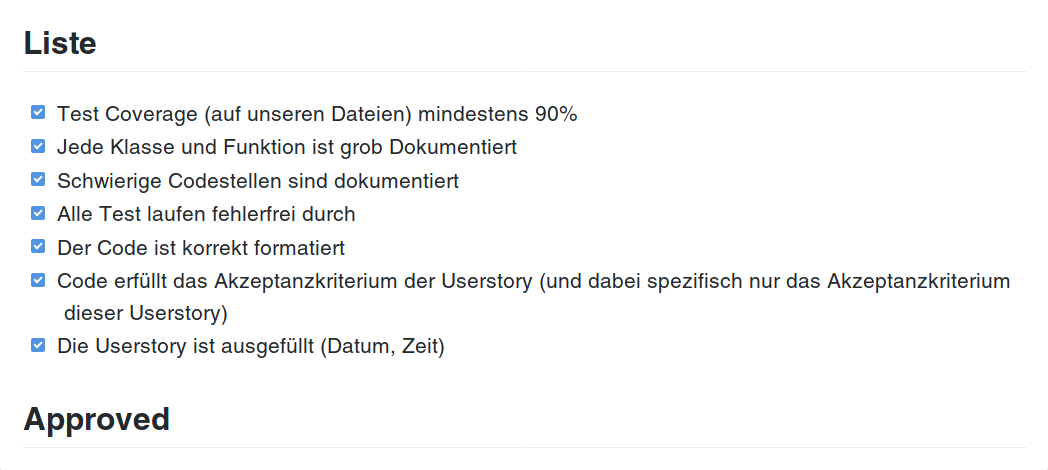
\includegraphics[width=.8\textwidth]{code_review/us26}
\caption{Review zur Userstory 26}
\end{figure}

\begin{figure}[H]
\centering
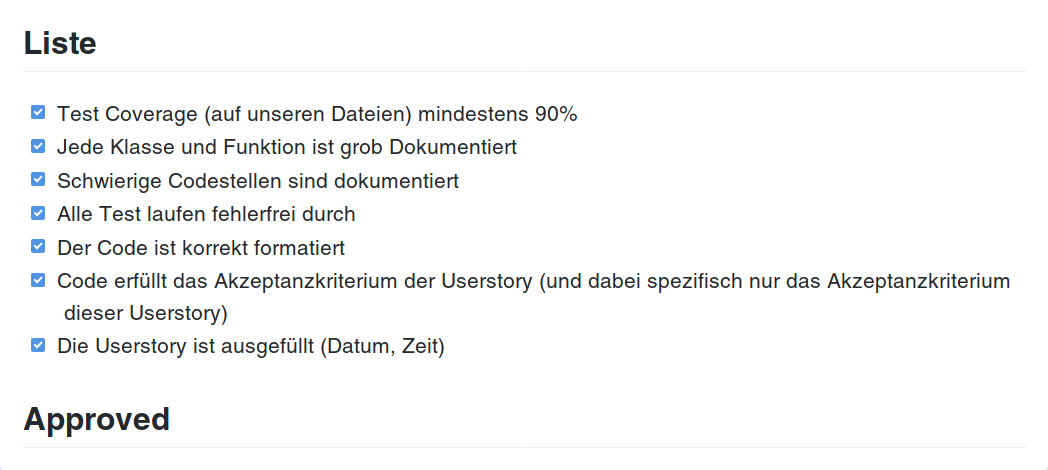
\includegraphics[width=.8\textwidth]{code_review/us27}
\caption{Review zur Userstory 27}
\end{figure}

\begin{figure}[H]
\centering
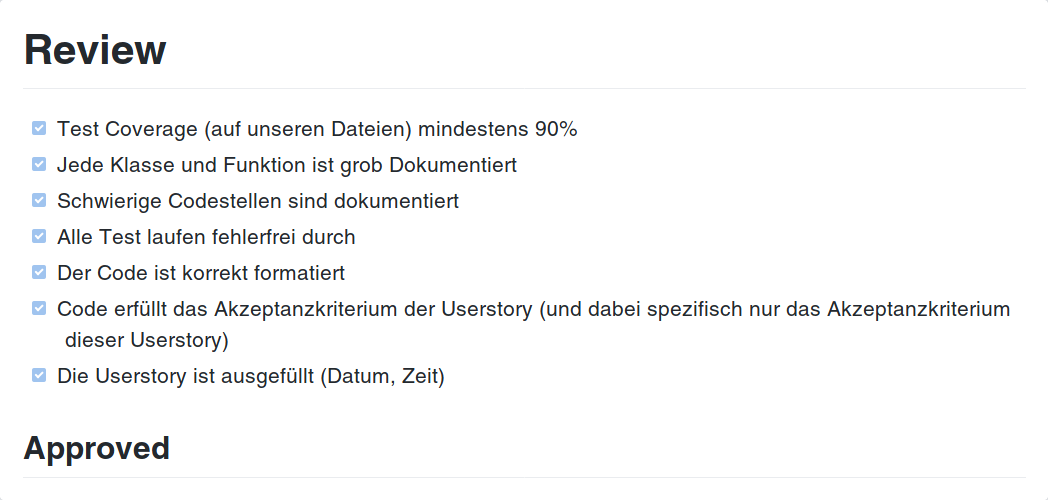
\includegraphics[width=.8\textwidth]{code_review/us28}
\caption{Review zur Userstory 28}
\end{figure}

\begin{figure}[H]
\centering
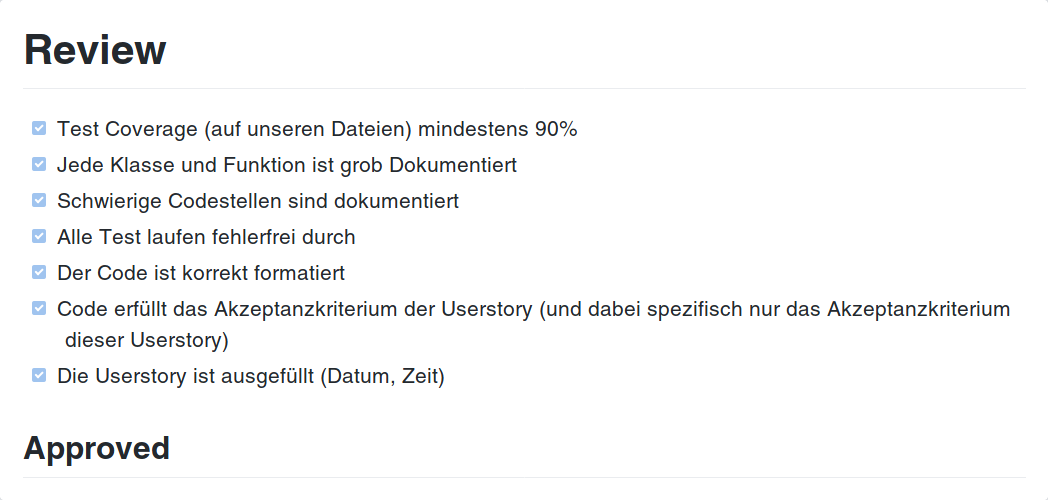
\includegraphics[width=.8\textwidth]{code_review/us29}
\caption{Review zur Userstory 29}
\end{figure}

\begin{figure}[H]
\centering
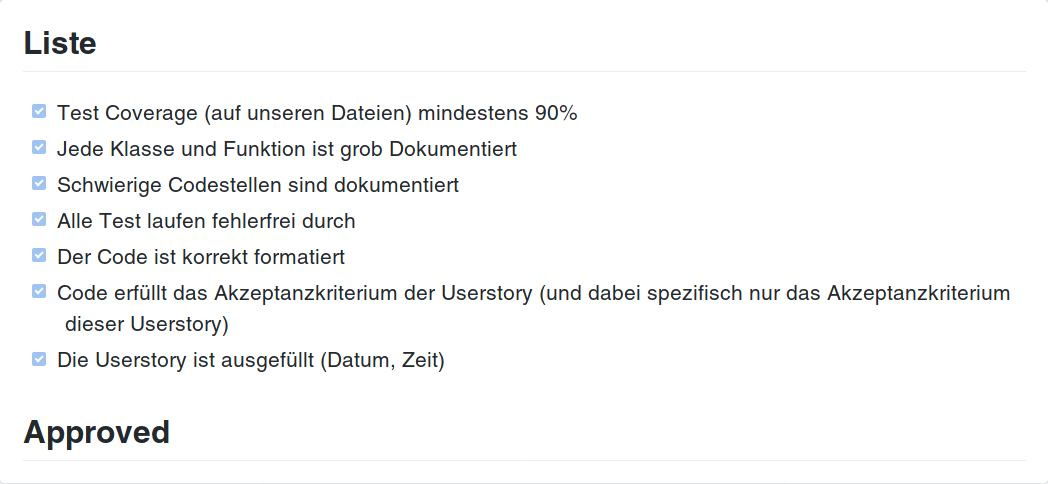
\includegraphics[width=.8\textwidth]{code_review/us30}
\caption{Review zur Userstory 30}
\end{figure}

\begin{figure}[H]
\centering
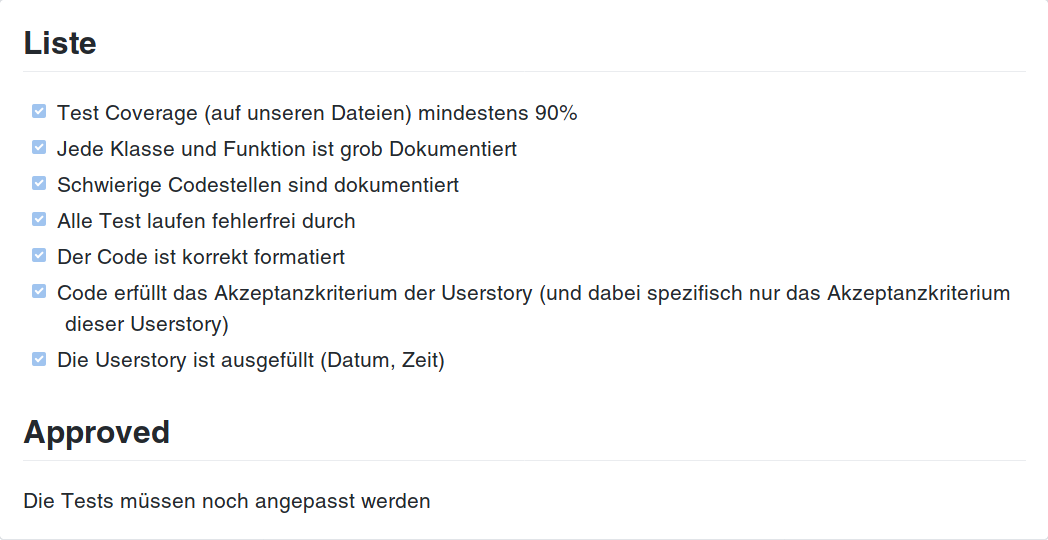
\includegraphics[width=.8\textwidth]{code_review/us31}
\caption{Review zur Userstory 31}
\end{figure}

\begin{figure}[H]
\centering
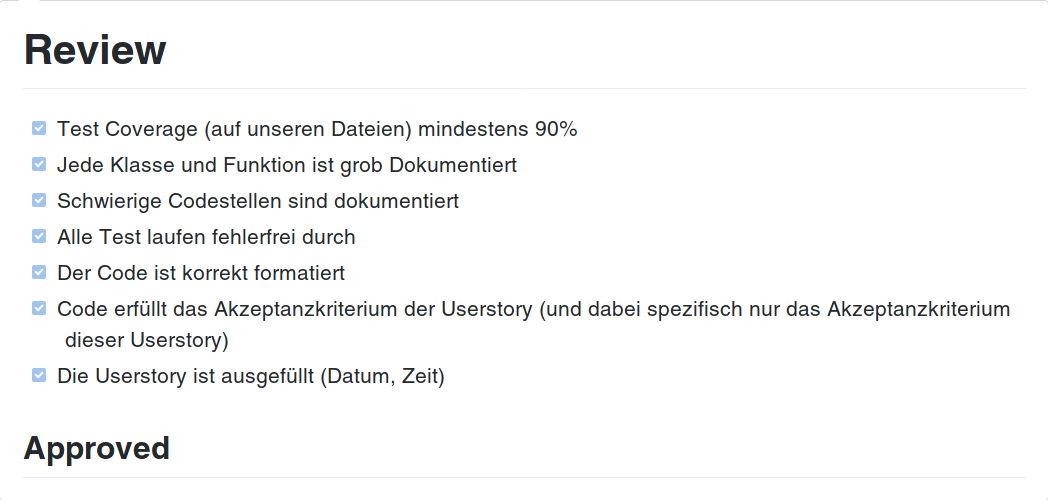
\includegraphics[width=.8\textwidth]{code_review/us32}
\caption{Review zur Userstory 32}
\end{figure}

\begin{figure}[H]
\centering
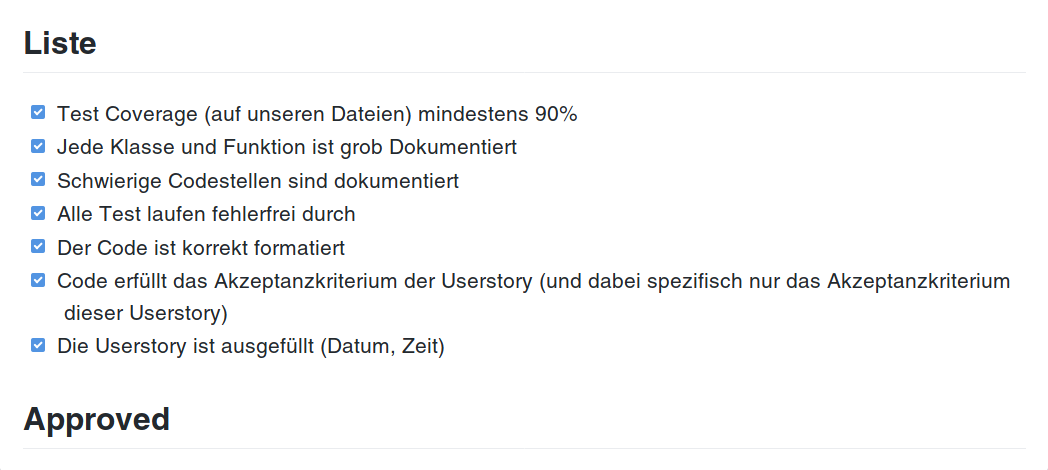
\includegraphics[width=.8\textwidth]{code_review/us33}
\caption{Review zur Userstory 33}
\end{figure}

\begin{figure}[H]
\centering
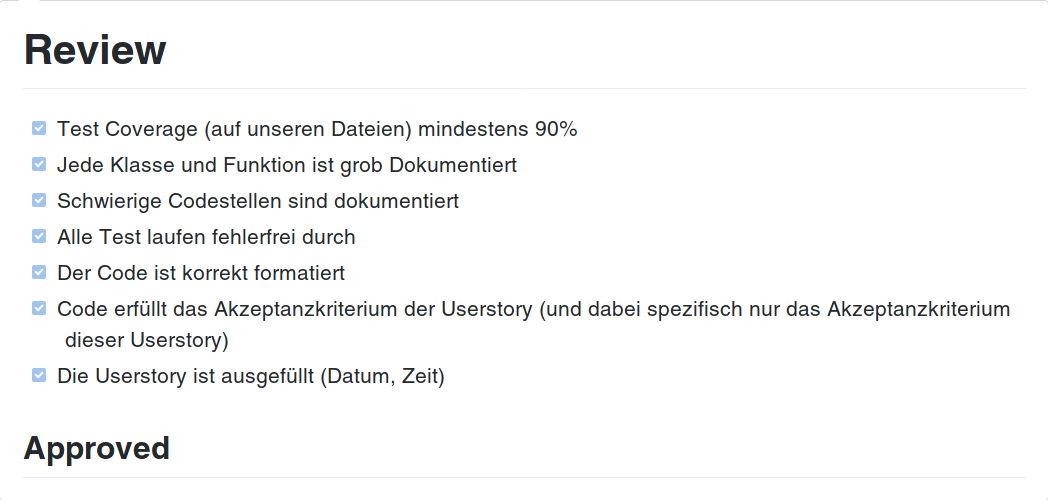
\includegraphics[width=.8\textwidth]{code_review/us34}
\caption{Review zur Userstory 34}
\end{figure}

\begin{figure}[H]
\centering
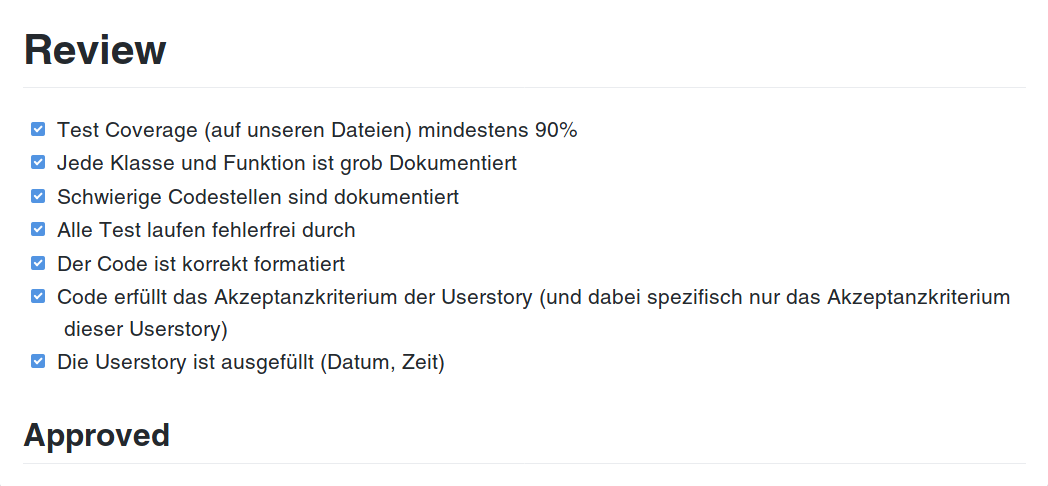
\includegraphics[width=.8\textwidth]{code_review/us35}
\caption{Review zur Userstory 35}
\end{figure}

\begin{figure}[H]
\centering
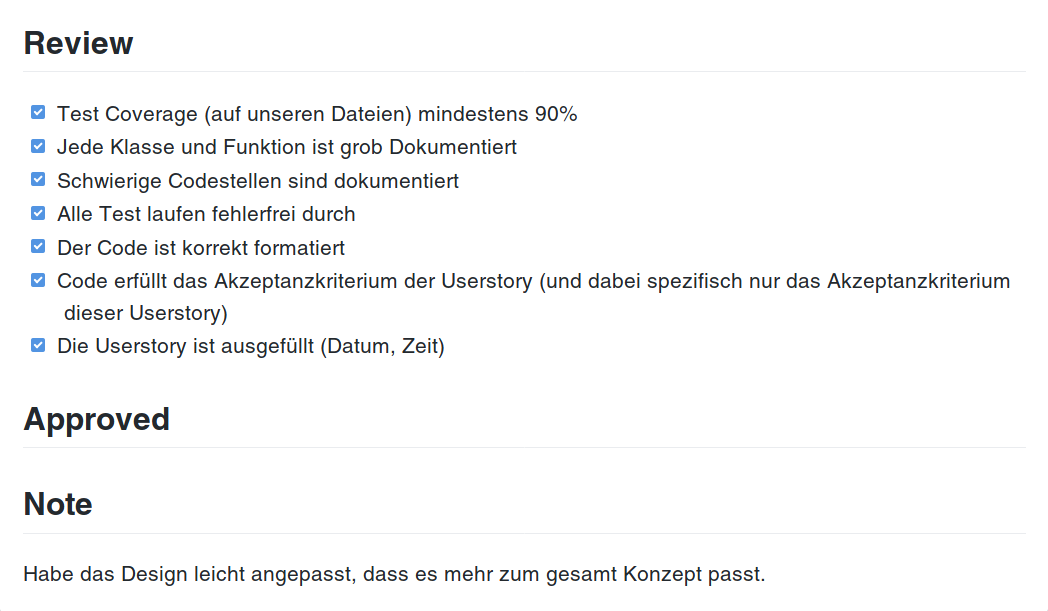
\includegraphics[width=.8\textwidth]{code_review/us36}
\caption{Review zur Userstory 36}
\end{figure}

\begin{figure}[H]
\centering
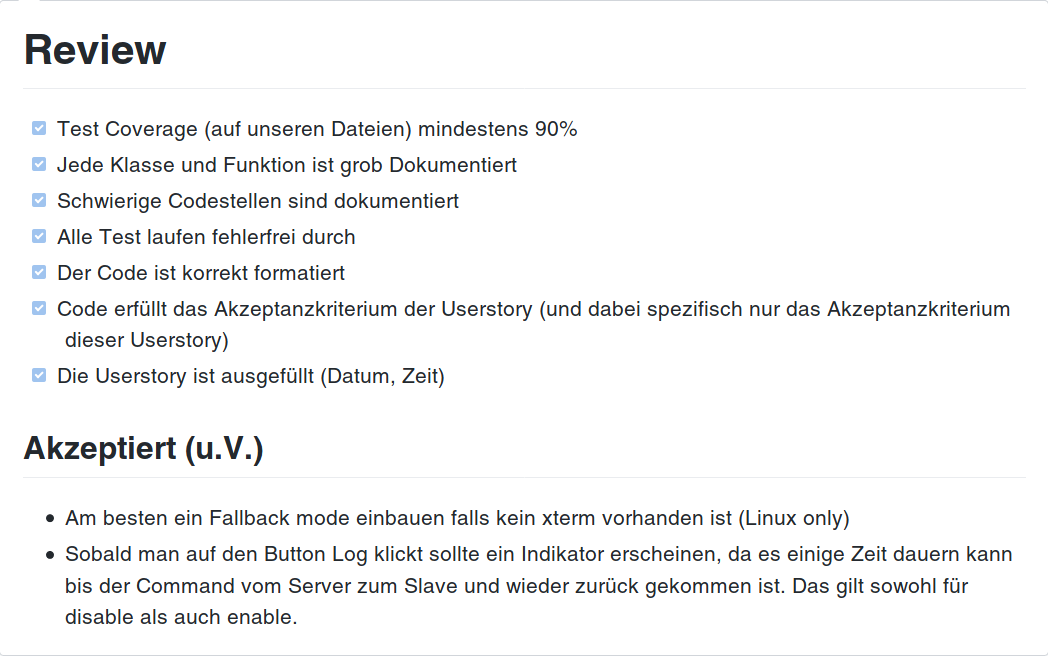
\includegraphics[width=.8\textwidth]{code_review/us37}
\caption{Review zur Userstory 37}
\end{figure}

\begin{figure}[H]
\centering
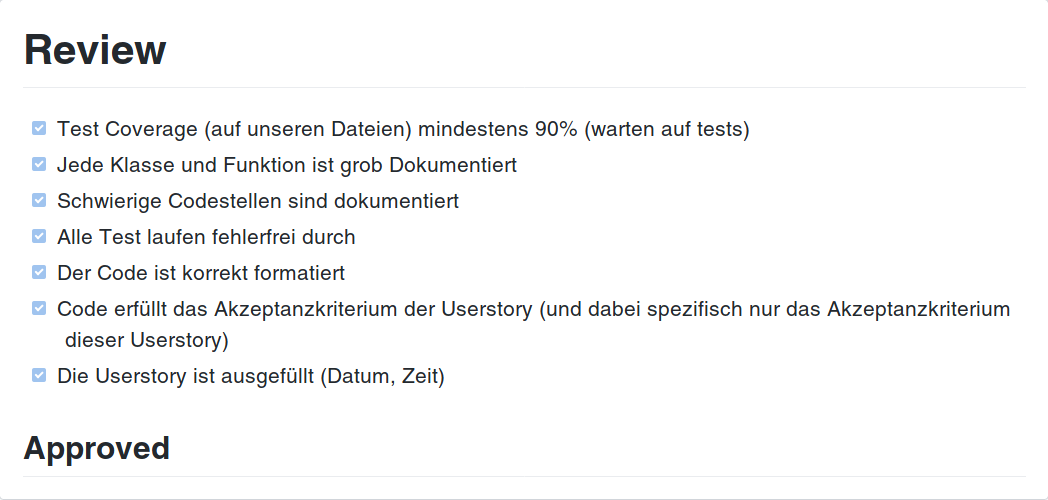
\includegraphics[width=.8\textwidth]{code_review/us38}
\caption{Review zur Userstory 38}
\end{figure}

\begin{figure}[H]
\centering
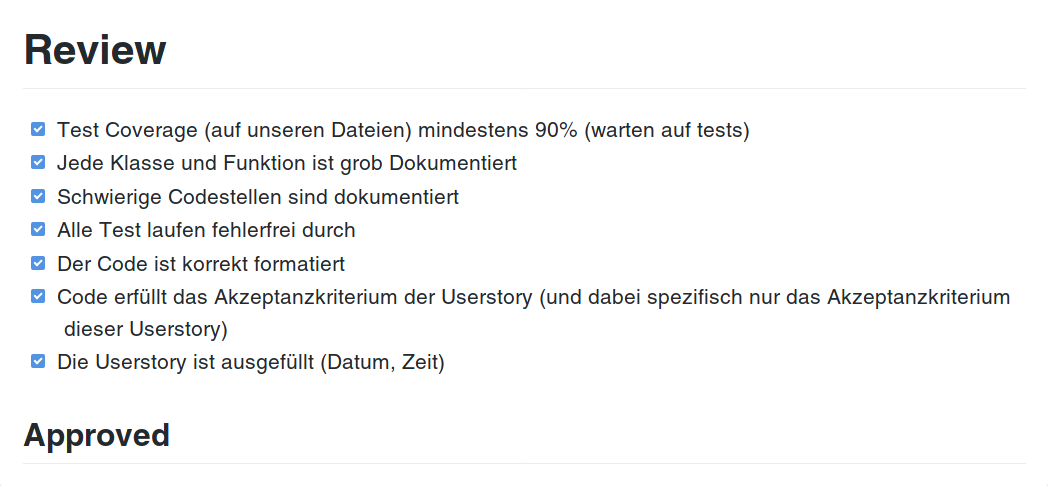
\includegraphics[width=.8\textwidth]{code_review/us39}
\caption{Review zur Userstory 39}
\end{figure}

\begin{figure}[H]
\centering
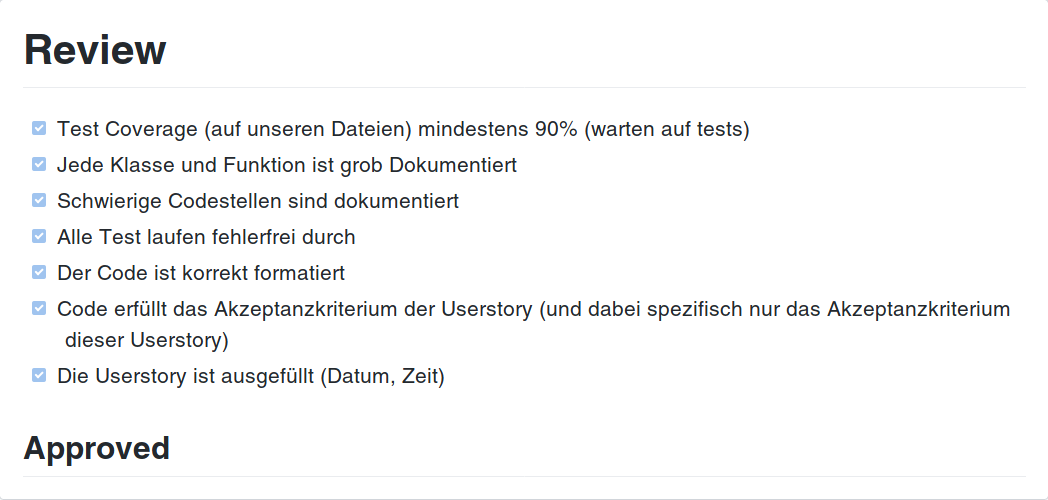
\includegraphics[width=.8\textwidth]{code_review/us40}
\caption{Review zur Userstory 40}
\end{figure}

\begin{figure}[H]
\centering
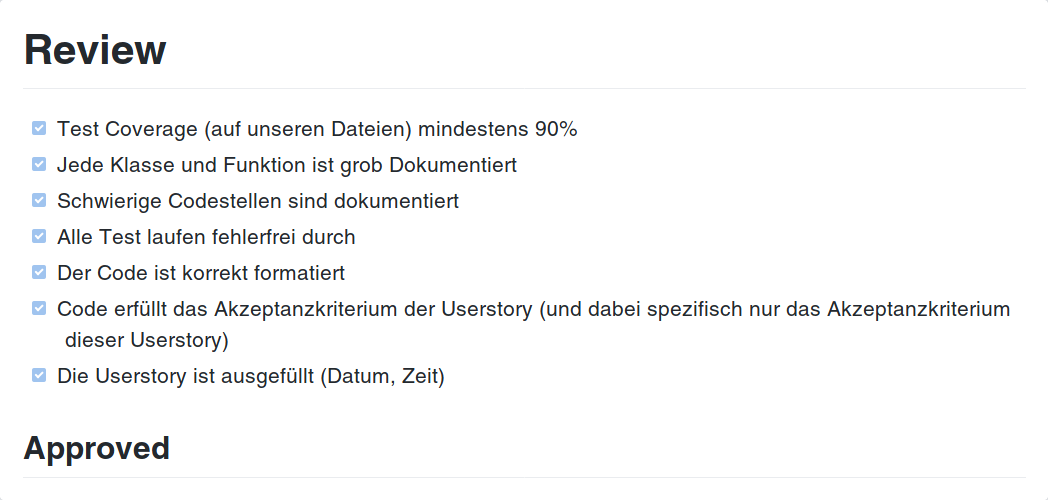
\includegraphics[width=.8\textwidth]{code_review/us41}
\caption{Review zur Userstory 41}
\end{figure}

\begin{figure}[H]
\centering
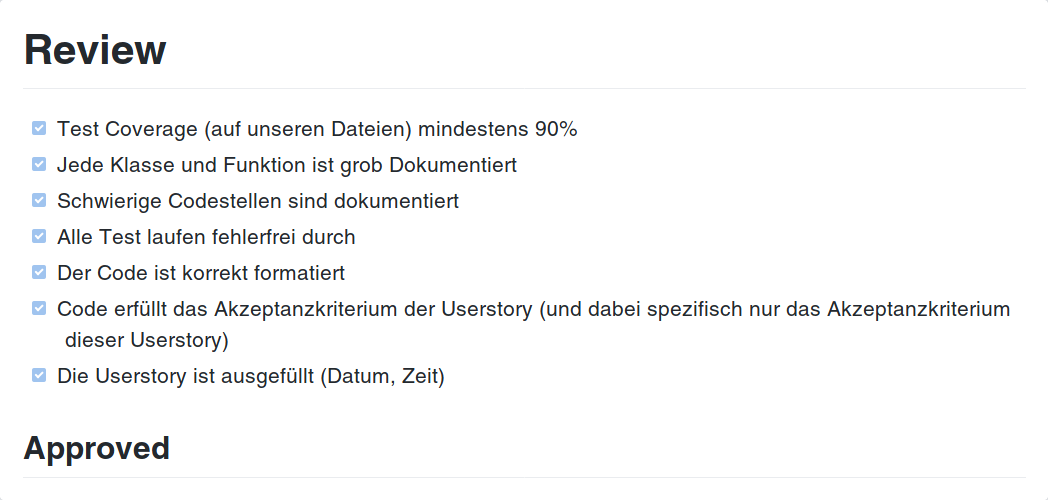
\includegraphics[width=.8\textwidth]{code_review/us42}
\caption{Review zur Userstory 42}
\end{figure}

\begin{figure}[H]
\centering
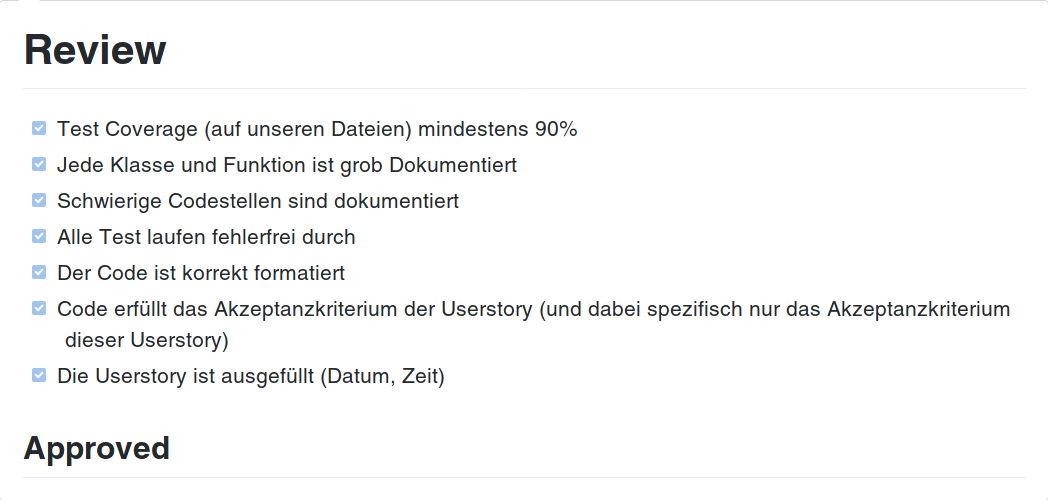
\includegraphics[width=.8\textwidth]{code_review/us43}
\caption{Review zur Userstory 43}
\end{figure}

\begin{figure}[H]
\centering
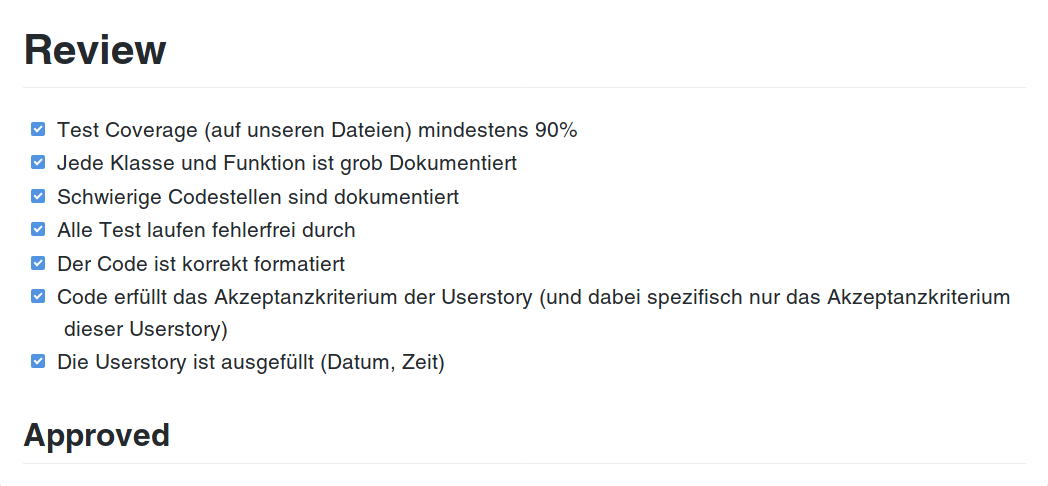
\includegraphics[width=.8\textwidth]{code_review/us44}
\caption{Review zur Userstory 44}
\end{figure}

\begin{figure}[H]
\centering
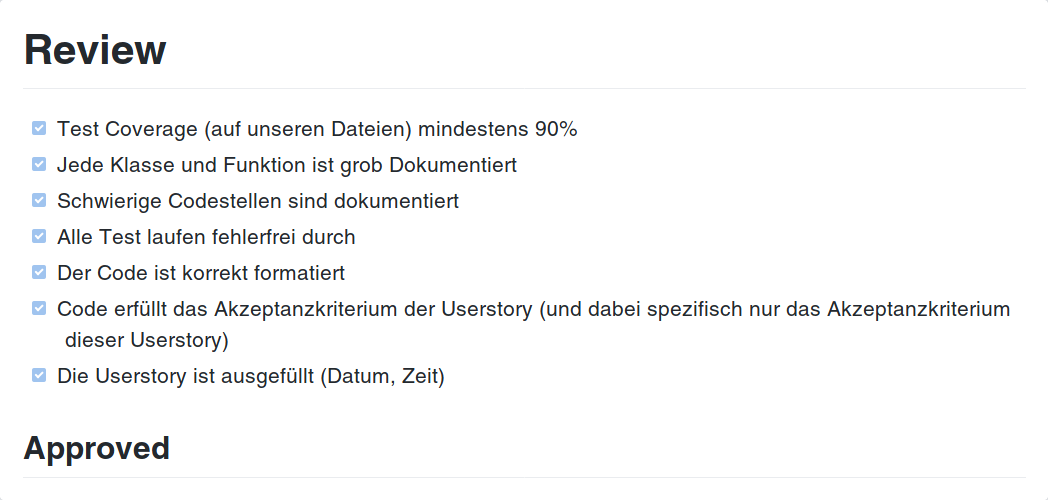
\includegraphics[width=.8\textwidth]{code_review/us45}
\caption{Review zur Userstory 45}
\end{figure}

\begin{figure}[H]
\centering
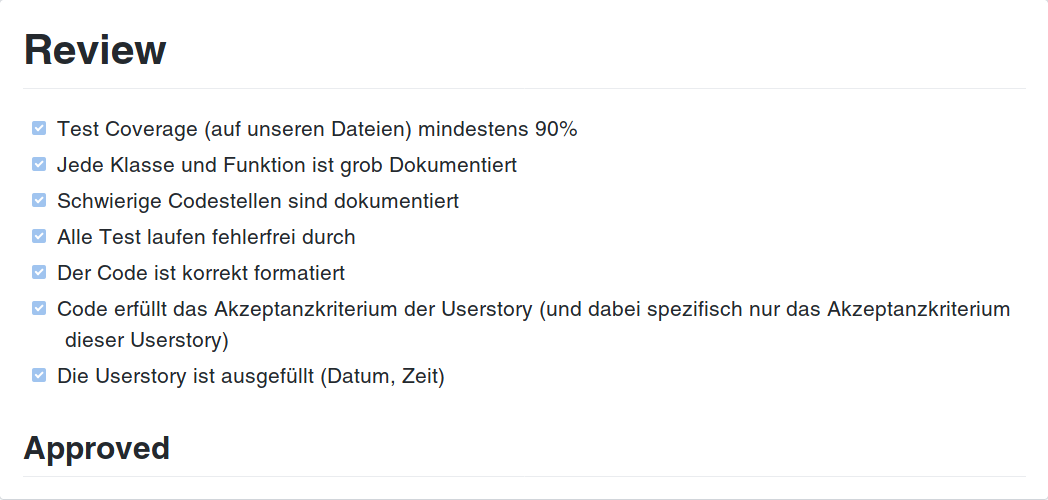
\includegraphics[width=.8\textwidth]{code_review/us46}
\caption{Review zur Userstory 46}
\end{figure}

\begin{figure}[H]
\centering
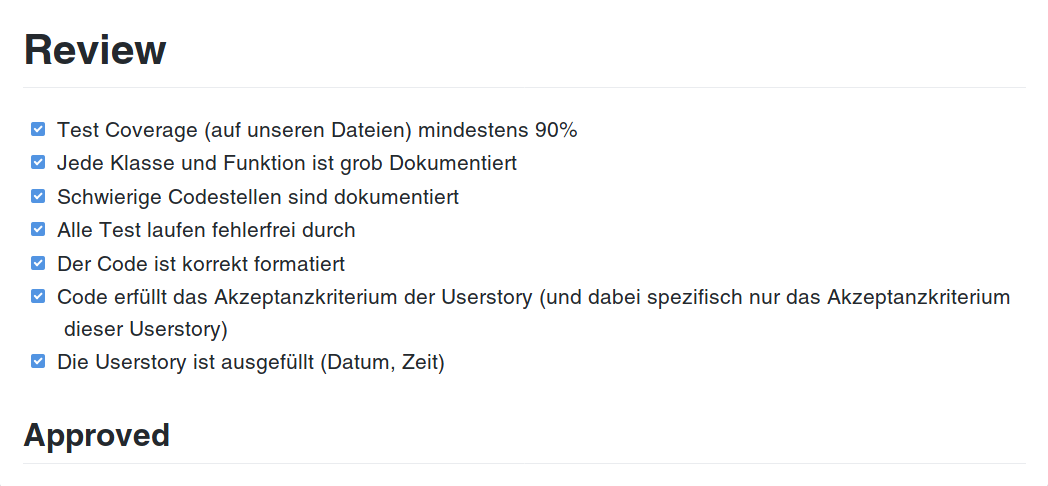
\includegraphics[width=.8\textwidth]{code_review/us47}
\caption{Review zur Userstory 47}
\end{figure}

\begin{figure}[H]
\centering
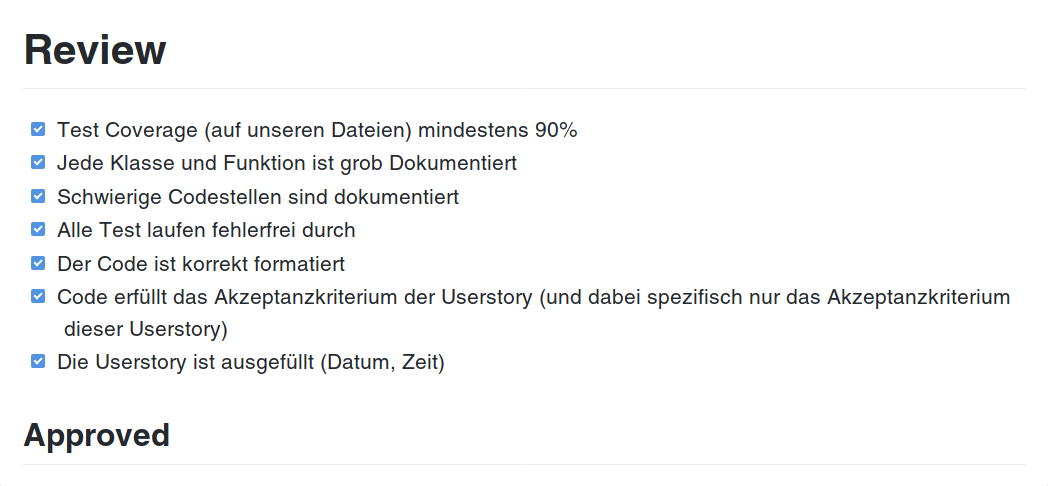
\includegraphics[width=.8\textwidth]{code_review/us48}
\caption{Review zur Userstory 48}
\end{figure}
